\documentclass[portrait]{sciposter}

\usepackage[utf8x]{inputenc}
\usepackage[ngerman, english]{babel}
\usepackage{amsmath}
\usepackage{amsfonts}
\usepackage{amssymb}
\usepackage{graphicx}
\usepackage{multicol}
\usepackage{sectionbox}

\author{Emile Hansmaennel}
\title{Development of components for\\ a ChiralSTEM -- Mode}
\institute{Universität Regensburg\\}
\email{andreas.hasenkopf@physik.uni-regensburg.de}
\leftlogo[1]{UniLogo2}
\rightlogo[1]{TEM-Logo}
\conference{14. European Microscopy Congress, Aachen, September 1--5, 2008}
\begin{document}

\maketitle
\rule{\textwidth}{2mm}

\begin{multicols}{3}

\begin{abstract}
The effect of \textbf{E}nergy-loss \textbf{M}agnetic \textbf{C}hiral \textbf{D}ichroism (EMCD) was proposed by Schattschneider et al. \cite{emcd_proposal} in analogy to XMCD due to similar scattering cross section expressions (wave vector transfer $\vec{q}$ in inelastic electron scattering $\leftrightarrow$ polarization vector $\vec{\epsilon}$ in X-ray absorption). The effect was measured for the first time by Rubino \cite{emcd_nature}.

The state of the art method for recording EMCD-spectra is the ''intrinsic method'' requiring the specimen to fulfill three strict properties (mono crystal, thickness, orientation) due to its use as a beam splitter. In order to avoid these requirements an alternative setup with a twin aperture and Boersch phase plate for generating 2 coherent electron waves with a phase difference of $\pi/2$ is suggested. Chiral contrast in energy-loss spectra is achieved due to a magnetic sample.

To determine whether a twin aperture is suitable for EMCD-measurements -- in particular in STEM-mode -- the wave function and intensity distribution in the sample plane are calculated numerically and the optimum dimensions for the aperture and phase plate are determined. Finally a STEM operation with a twin aperture is realized.
\end{abstract}

\section{Intrinsic method}
\textbf{\scshape Analogon to Circular Polarization}: two scattered coherent electron waves (wave vector transfers: $q_1$, $q_2$, $q_1\perp q_2$ or $q\,'_1$, $q\,'_2$, $q\,'_1\perp q\,'_2$) with a phase difference of $\pi/2$.

\begin{figure}[h]
\begin{center}
\label{fig_intrinsic}
\includegraphics[width=\textwidth]{poster_aperture_einzel.png}
\caption{setup -- intrinsic method}
\end{center}
\end{figure}

\textbf{\scshape Setup}: see fig. \ref{fig_intrinsic}.
\begin{itemize}
\item proposed by Nelhiebel \cite{emcd_intrinsic} and used in prior EMCD-measurements\cite{emcd_nature,pd_rubino,pd_hurm},
\item mono crystalline sample as beam splitter,
\item two Bragg reflexes with phase difference $\pi/2$ in the diffraction plane according to dynamic diffraction theory (see \cite{pd_rubino,pd_hurm}).
\end{itemize}

\textbf{\scshape Deficiencies}:
\begin{itemize}
\item signal low,
\item resolution low (improved by convergent beam technique \cite{mcd_in_eels_2}),
\item long duration of measurement.
\end{itemize}

\textbf{\scshape Needed Improvements}:
\begin{itemize}
\item higher intensity within
\item small specimen area
\item[$\Rightarrow$] focussed beams $\to$ STEM?!
\end{itemize}

\section{Twin Aperture}
\textbf{\scshape Suggestion}: see fig. \ref{fig_twin}
\begin{itemize}
\item twin aperture $\to$ two coherent partial electron waves,
\item condenser lens $\to$ focussing,
\item electrostatic Boersch phase plate (annular electrode) \cite{phaseplate} $\to$ application of phase shift to one partial wave
\end{itemize}

\begin{figure}[h]
\begin{center}
\label{fig_twin}
\includegraphics[width=\textwidth]{poster_aperture_twin.png}
\end{center}
\caption{setup -- twin aperture}
\end{figure}
% one electron wave is shifted in phase such that the phase difference of the two waves in the sample plane is $\pi/2$ and such that a similar diffraction pattern is observed in the diffraction plane as for the intrinsic method.

%Therefor the possibility of a STEM operation with such a twin aperture was investigated due to the wish to perform EMCD measurement in a STEM mode in the future.

\section{Numerical Calculations}

\textbf{\scshape Intensity Distribution}: $|\psi_{BFP}|^2$, see fig. \ref{fig_linescan}
\begin{eqnarray}
\psi_{BFP}(X,\,Y) &=& \mathrm{J}_1\left(\frac{2\pi R\sqrt{X^2+Y^2}}{\lambda f}\right)\frac{\lambda f}{\pi R\sqrt{X^2+Y^2}} \nonumber \\
&& \cdot\left( e^{-\frac{id_1X}{\lambda f}}+e^{-\frac{id_2X}{\lambda f}-i\varphi}\right),\nonumber \\
\Delta\phi(X) &=& \left((d_2-d_1)\frac{X}{\lambda f}+\varphi+\pi\right)\mathrm{mod}(2\pi)-\pi \nonumber
\end{eqnarray}

\begin{itemize}
\item in sample plane $\equiv$ back focal plane (BFP)
\item influence of phase shift on intensity in BFP
\item what are optimum parameters for $R$, $d_1$, $d_2$ and $\varphi$?
\end{itemize}

\begin{figure}[h]
\includegraphics[width=\textwidth]{poster_linescan.png}
\caption{intensity distribution and phase difference}
\label{fig_linescan}
\end{figure}

%As one can see the maximum of the intensity distribution and the $\pi/2$-polygon coincide. Thus it is possible to adjust a phase shift to one electron wave such that the phase difference in the BFP reaches it's optimum value of $\pi/2$ at the maximum of the intensity distribution in the BFP.

\textbf{\scshape Definition}: quality parameter $U$ and weighting function $\Upsilon$:
\begin{eqnarray}
\label{eqn_usignal}
U &=& \frac{\int\limits_{-\infty}^\infty\Upsilon(X)|\psi_{BFP}(X,\,0)|^2\,\mathrm{d}X}{\int\limits_{-\infty}^\infty|\psi_{BFP}(X,\,0)|^2\,\mathrm{d}X} \nonumber\\
\label{eqn_upsilon_1}
\Upsilon(X) &=& 2\,\mathrm{sgn}\left(\Delta\phi(X)\right)\left|\left(\frac{\Delta\phi(X)}{\pi}+\frac{1}{2}\right)\mathrm{mod}\,1-\frac{1}{2}\right| \nonumber\\
\label{eqn_sn}
\mathrm{S/N} &=& \frac{\int\limits_a^b|\psi_{BFP}(X,\,0)|^2\,\mathrm{d}X}{\int\limits_{-\infty}^\infty|\psi_{BFP}(X,\,0)|^2\,\mathrm{d}X},\;[a,\,b]: \mathrm{FWHM} \nonumber
\end{eqnarray}

\begin{itemize}
\item $U$: coarse measure for percentage of intensity with  phase difference $= \pi/2$ ,
\item S/N: ratio between intensity within FWHM and total intensity,
\item $\Upsilon$: zigzag weighting function (see fig. \ref{fig_upsilon}) defined to fulfill:

\begin{equation}
\Upsilon(X) = \left\{\begin{array}{rcl}
\pm1 &\mathrm{for}& \Delta\phi(X) = \pm\frac{\pi}{2} \\
0 &\mathrm{for}& \Delta\phi(X) = i\pi,\;i=0,\,\pm1 \\
\end{array}\right. .\nonumber
\end{equation}
\end{itemize}

\textbf{\scshape Optimum Parameter Set}: determined by brute-force method
\begin{itemize}
\item numerical calculation: $U$, FWHM and S/N for each parameter set,
\item saving results in MySQL database $\to$ graphical evaluation: fig. \ref{fig_sql_1} and \ref{fig_sql_2}
\item[$\Rightarrow$] \textbf{aperture}: maximum radius and minimum spacing
%(see fig. \ref{fig_linescan})
\item[$\Rightarrow$] chosen parameters: Radius = $28.5\mu$m, Spacing = $60.7\mu$m, Phase shift = $0.57\pi$
\end{itemize}

\begin{figure}[h]
\begin{center}
\includegraphics[width=\textwidth]{poster_upsilon.png}
\end{center}
\caption{weighting function $\Upsilon$ (for legend see fig. \ref{fig_linescan})}
\label{fig_upsilon}
\end{figure}

%whereby $J_1$ is the Bessel function, $\Delta\phi$ is the phase difference between two electron waves in the diffraction plane, $X$ is an coordinate in that plane, $d_{1,2}$ are the spacings of the apertures' centers from the optical axis, $R$ is the aperture radius, $\lambda$ is the electron wave length, $f$ is the focal length of the lens and $\varphi$ is the phase shift due to a phase plate.

\begin{figure}[hbt]
\label{fig_sql_1}
%\includegraphics[width=.8\textwidth]{poster_sql_u.png}
\includegraphics[width=\textwidth]{poster_usignal_2.png}
\caption{evaluation -- $U$}
\end{figure}

\begin{figure}[hbt]
%\includegraphics[width=.8\textwidth]{poster_sql_sn.png}
\includegraphics[width=\textwidth]{poster_sn_2.png}
\caption{evaluation -- Signal/Noise (for legend see fig. \ref{fig_sql_1})}
\label{fig_sql_2}
\end{figure}

%The data sets generated in this way are stored in a MySQL database and are plotted in dependence of the spacing between the apertures in figures \ref{fig_sql_1} and \ref{fig_sql_2}. Figure \ref{fig_sql_1} shows the dependence of the quantity $\mathfrak{U}$ and figure \ref{fig_sql_2} the dependence of the S/N ratio for different aperture radii (7, 11, 17, 21 and 27 $\mu$m) on the aperture spacing.

%These results suggest the use of large aperture radii but small aperture spacings. According to that the parameters given in the legend of figure \ref{fig_linescan} (Radius: 28$\mu$m, Spacing: 62$\mu$m) were chosen further regarding the available area on the used SiN membrane for production of a twin aperture.

\section{Experiments}
\textbf{\scshape Production}: electron lithography
\begin{itemize}
\item holes in SiN membrane (100$\mu$m$\times$100$\mu$m)
\item evaporation of gold
\end{itemize}

\textbf{\scshape STEM}: operation with condenser twin aperture
\begin{itemize}
\item sample: gold particles on a carbon foil.
\item comparison: conventional aperture $\leftrightarrow$ twin aperture
\item[$\Rightarrow$] no influence on image quality
\end{itemize}

\begin{figure}[hbt]
\label{fig_goldstem}
\subfigure[twin aperture]{\label{fig_goldstem_a}
%\includegraphics[width=.475\textwidth]{gold_einzel_50k.png}
\includegraphics[width=.45\textwidth]{8061-5png.png}}
\subfigure[STEM image]{\label{fig_goldstem_b}\includegraphics[width=.45\textwidth]{gold_twin_50k.png}}
\caption{twin aperture (w/o phase plate) \& STEM image of gold particles using twin aperture.}
\end{figure}

%Figure \ref{fig_goldstem} shows images observed in STEM-mode with the CM30 at a magnification of $5\cdot10^4$. By means of red arrows two particles are marked in both figures. Figure \ref{fig_goldstem}(a) shows the image obtained with an einzel aperture and \ref{fig_goldstem}(b) the image obtained using the twin aperture.

%As one can see the use of a twin aperture has no apparent negative influence on image quality.

\section{Outlook}
\begin{multicols}{2}
\textbf{\scshape Electron Lithography}: phase plate
\begin{itemize}
\item negative resist PMMA\cite{pmma}
\item[$\Rightarrow$] deposition of gold $\to$ annular electrode
\item deposition of insulating layers and gold overlays
\end{itemize}
\textbf{\scshape EMCD}: record spectra in
\begin{itemize}
\item diffraction mode
\item STEM-mode
\end{itemize}
\end{multicols}

\begin{multicols}{2}
\tiny
\bibliographystyle{plain}
\bibliography{literature}
\end{multicols}

\end{multicols}
\end{document}

% \documentclass[a2,landscape]{a0poster}
%
% \usepackage{multicol}
% \columnsep=100pt
% \columnseprule=3pt
%
% \usepackage[svgnames]{xcolor}
%
% \usepackage{times} % Times New Roman
% \usepackage{graphicx} % Required for including images
% \graphicspath{{figs/}} % Location of the graphics files
% \usepackage{booktabs} % Top and bottom rules for table
% \usepackage[font=small,labelfont=bf]{caption} % Required for specifying captions to tables and figures
% \usepackage{amsfonts, amsmath, amsthm, amssymb} % For math fonts, symbols and environments
% \usepackage{wrapfig} % Allows wrapping text around tables and figures
%
% \usepackage[english,ngerman]{babel}
% \usepackage[utf8]{inputenc}
%
% \begin{document}
%
% % Header | 55% | 25% | 19% |
%
% \begin{minipage}[b]{0.45\linewidth}
% \veryHuge \color{NavyBlue} \textbf{Galaxy Generation} \color{Black}\\ % Title
% \Huge\textit{Visualizierung und Generierung von Galaxien}\\[1cm] % Subtitle
% \huge \textbf{Emile Hansmaennel}\\ % Author(s)
% \huge Theodor Fliedner Gymnasium\\ % University/organization
% \end{minipage}
% %
% \begin{minipage}[b]{0.35\linewidth}
%   
\includegraphics[height=7.5cm]{logos}
%   \vspace{5cm}
% \end{minipage}
% %
% \begin{minipage}[b]{0.19\linewidth}
% 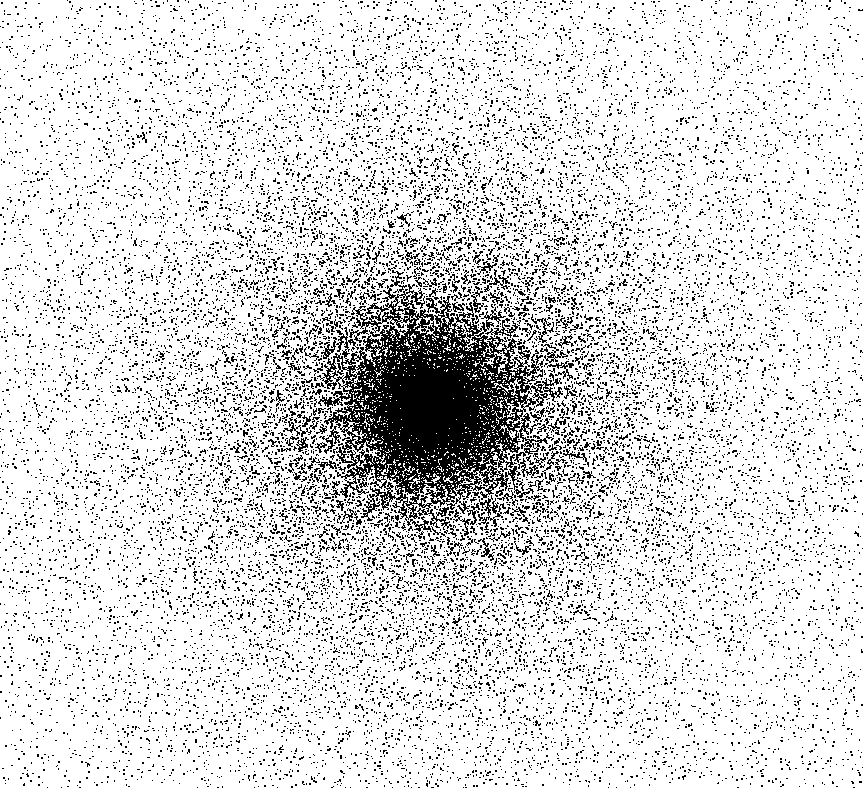
\includegraphics[height=15cm]{galaxy} % Logo or a photo of you, adjust its dimensions here
% \end{minipage}
%
% \vspace{1cm} % A bit of extra whitespace between the header and poster content
%
% %----------------------------------------------------------------------------------------
%
% \begin{multicols}{4} % This is how many columns your poster will be broken into, a poster with many figures may benefit from less columns whereas a text-heavy poster benefits from more
%
% %----------------------------------------------------------------------------------------
% %	ABSTRACT
% %----------------------------------------------------------------------------------------
%
% \color{Navy} % Navy color for the abstract
%
% \begin{abstract}
%
%   Das Ziel meines Projektes ist es, Realitätsgetreue Galaxien und Dunkle Materie
%   Halos zu generieren.
%   Hierzu verwende ich das sogenannte ''Navarro-Frenk-White'' Profil welches in
%   Kombination mit der ''Random Sampling'' Methode die Dichteverteilung
%   der Sternenpositionen in Koordinaten für einzelne Sterne umgewandelt.
%   \par
%   Vergleicht man die generierten Galaxien mit echten Galaxien fällt auf das
%   die Sterne sich anders verhalten. Dies lässt sich durch Dunkle Materie erklären,
%   welche man jedoch nicht direkt beobachten kann. Es kann also
%   nur aufgrund ihrer Auswirkungen auf andere Objekte auf sie geschlossen werden,
%   weshalb es nicht ganz Trivial ist sie sichtbar darzustellen.
%   \par
%   Im Verlauf des Projektes haben sich mir jedoch auch andere Teilbereiche
%   eröffnet wie z. B. die Generation von Spiralgalaxien, die Optimierung von
%   Rechenprozessen und die Nutzung von einem neuronalen Netz zur Anpassung der
%   generierten Galaxie an eine reale Galaxie.
%
% \end{abstract}
%
% %----------------------------------------------------------------------------------------
% %	INTRODUCTION
% %----------------------------------------------------------------------------------------
%
% \color{SaddleBrown} % SaddleBrown color for the introduction
%
% \section*{Einleitung}
%
% Das Hauptziel des Projektes war es, Galaxien dreidimensional darzustellen um
% diese mit echten Galaxien vergleichen zu können. Dies ist vorallem interessant,
% um echte real vorhandene Galaxien zu untersuchen, da man diese nur aus einer
% Perspektive beobachten kann (von der Erde aus).
% \par
% Dazu verwendete ich die sogennante Random-Sampling-Methode um aus einer
% Warscheinlichkeitsverteilung (dem Narvarro-Frenk-White Profil) Koordinaten
% zu generieren.
% \par
% Ein wichtiger Aspekt der beim generieren von Galaxien ist die Effizienz des
% verwendeten Programms extrem stark zu erhöhen, sodass in einer vergleichsweisen
% geringen Zeit, z.B. sehr viele Sterne generiert werden können. Um dies zu
% erreichen können sehr viele verschieden Ansätze mit eingebracht werden wie
% zum Beispiel die nutzung von mehreren sogennanten "Threads`` zum parralellisieren
% der Rechenarbeit.
% \par
% Um die genauigkeit der generierten galaxie im vergleich zu echten galaxien
% zu erhöhen, können Neuronale Netze verwendet werden. Diese beanspruchen jedoch
% sehr viel Rechenarbeit weshalb sich ihre nutzung erst in ein paar Jahren
% lohnen wird.
% \par
% Das Generieren von Spiralgalaxien führt ebenfalls zu einem Problem: der
% Rechenaufwand steigt mit der Anzahl der Sterne proportional exponentiall an.
% Die Lösung dieses Problems führt zu einer unterteilung der Galaxie in
% verschiedene Zellen, in denen die Kräfte gemittelt werden und anschließend mit
% den anderen Zellen interagieren.
%
% %----------------------------------------------------------------------------------------
% %	OBJECTIVES
% %----------------------------------------------------------------------------------------
%
% \color{DarkSlateGray} % DarkSlateGray color for the rest of the content
%
% \section*{Hauptziele}
%
% \begin{enumerate}
% \item Generieren von Elliptischen Punktwolken mithilfe des Narvarro-Frenk-White
% profils in verbindung mit der Random-Sampling Methode
%
% \item Verbesserung des Generierungsprozesses mithilfe von "Threadding``
%
% \item Generierund von Dunkle-Materie-Halos
%
% \item Nutzung von Neuronalen Netzen zum unbeaufsichtigten generieren von
% Galaxien
% \end{enumerate}
%
% %----------------------------------------------------------------------------------------
% %	MATERIALS AND METHODS
% %----------------------------------------------------------------------------------------
%
% \section*{Materialien und Methoden}
%
% Die verwendete Hardware die zum erstellen der Skripte wervendet wurde war ein
% Acer Laptop mit 2 Rechenkernen welche jeweils 2 Threads enthalten und mit bis
% zu 3,1 GHZ Takten. Die Simulationen wurden während des Praktikums in Heidelberg
% auf dem Laptop im kleinen stil getestet und anschließen auf einem Cluster marke
% eigenbau über einen längeren Zeitraum laufen gelassen. Im Cluster befanden sich
% ca. 14 Rechner mit wahlweise 4 oder 6 Kernen welche ebenfalls alle
% Hyperthreading unterstützten. Nach dem Praktikum verwendete ich zum großteil
% den Laptop und einen Server der mir von einem Freund gestellt wurde. Dieser
% verfüht über 2 mal 6 Kerne die ebenfalls Hyperthreading unterstützen was zu
% 24 logischen Prozessoren mit einer Taktrate von 2,5 GHZ führt.
%
% \par
%
% Zum generieren der Punktwolken verwendete ich das NFW-Profile in kombination
% mit der Random Sampling Methode wodurch die potentielle Koordinaten von Sternen
% entweder akzepriert oder verworfen wurden. Die Koordinated wurden in einer
% .csv Datei gespeichert welche von einem anderem Script weiterverwendet wurde um
% die Sterne in der 3D-Software Suite Blender darzustellen.
% Die Generierung von Spiralgalaxien ist (zurzeit) zu anspruchsvoll, weshalb die
% Daten aus der Punktwolke nicht genutzt werden können, da die quantitative Menge
% zu groß ist. Es wird deshalb eine andere Galaxie mit weniger Sternen generiert.
%
% %------------------------------------------------
%
% \subsection*{Random Sampling des Narvarro Frenk White Profils}
%
% Das Navarro-Frenk-White Profile (NFW-Profile) wird dazu genutzt, einem Stern
% in einem Abstand \( r \) vom Mittelpunkt der Galaxie eine Warscheinlichkeit
% \( \rho(r) \) zuzuweisen. Diese Warscheinlichkeit ist in Abbildung
% \ref{fig:lookup_NFW} in abhängigkeit zur Entfernung des Mittelpunkt der Galaxie
% dargestellt.
%
% \begin{center}%\vspace{0.5cm}
% \begin{equation*} \label{eq:NFW_profile}
%   \rho_{NFW}(r) = \frac{ 1 }{ \sqrt{ 2 \pi } \cdot \sigma } \cdot
%   \exp \left( \frac{ -\phi(r) }{ \sigma^{ 2 } } \right)
% \end{equation*}
%
% \begin{equation*}
%   \phi(r) = \frac{ 4\pi \cdot G \cdot f_{0} \cdot R_{s}^3 }{ r } \cdot
%   ln{ \left( 1 + \frac{ r }{ R_{s} } \right) }
% \end{equation*}
% \end{center}%\vspace{0.5cm}
%
% \begin{center}\vspace{0.5cm}
% 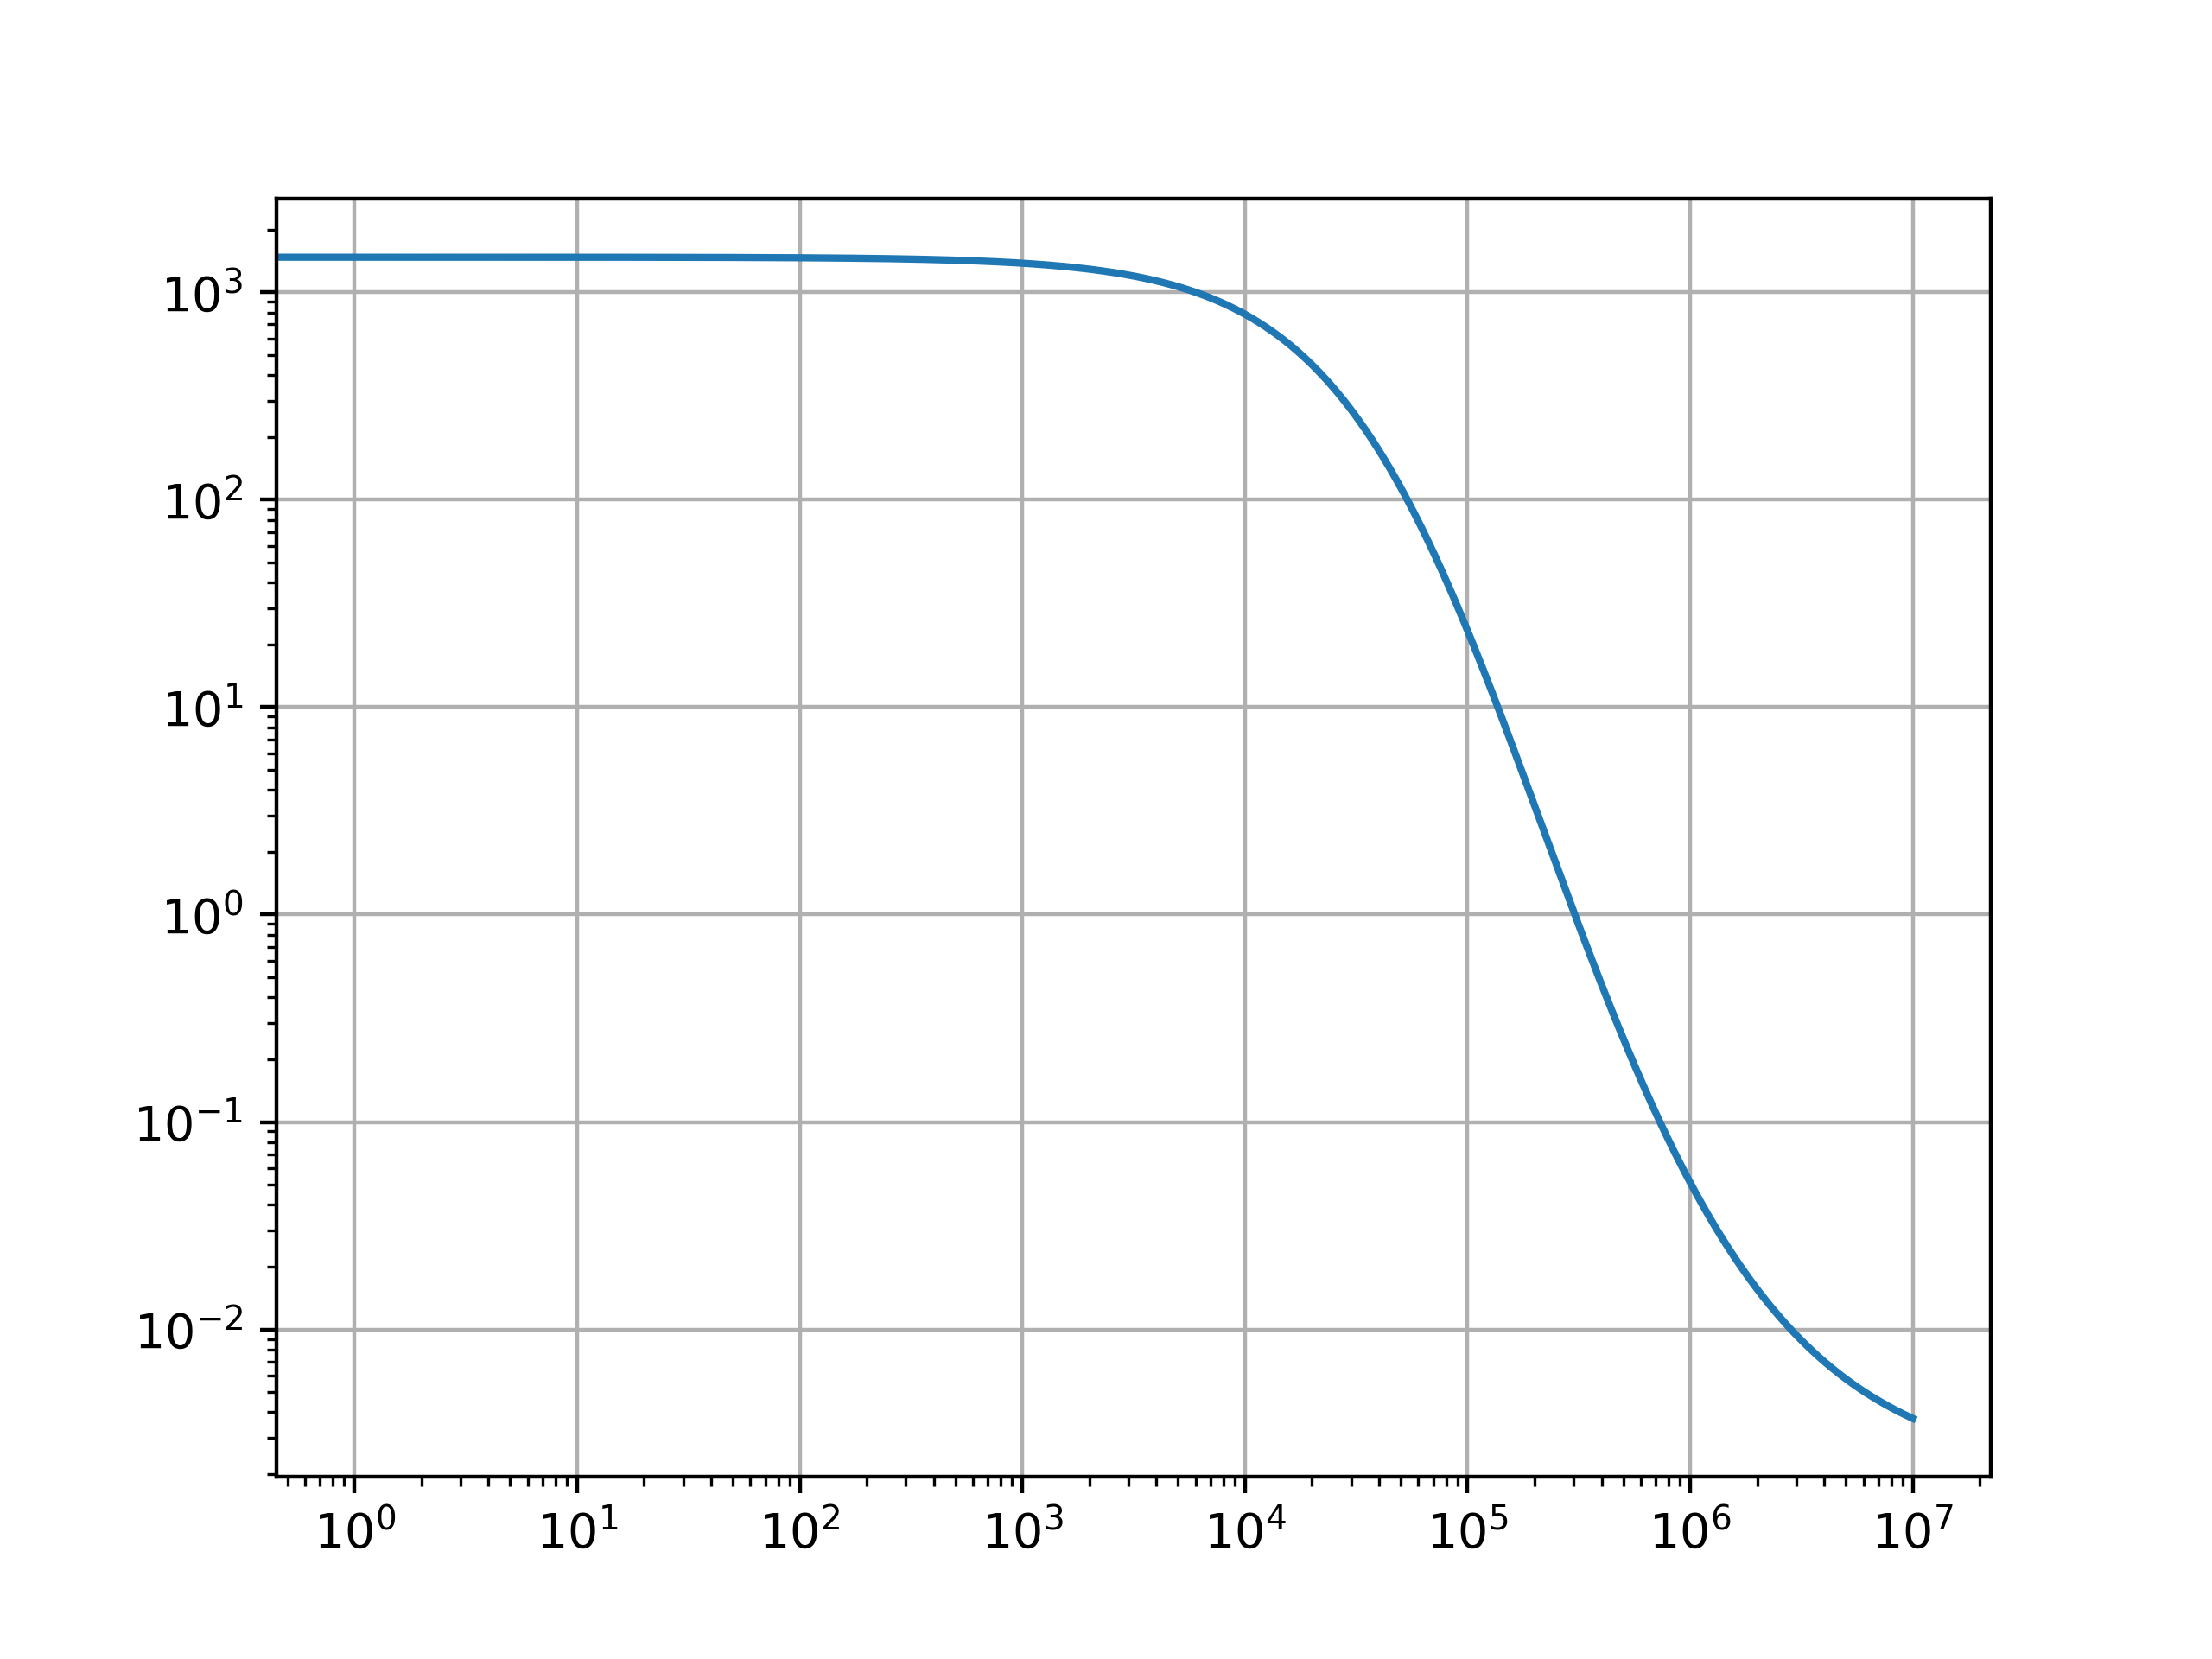
\includegraphics[width=0\linewidth]{1e6_6}
% \captionof{figure}{Das Navarro-Frenk-White Profile}
% \label{fig:equation_NFW}
% \end{center}\vspace{0.5cm}
%
% \begin{center}\vspace{0.5cm}
% 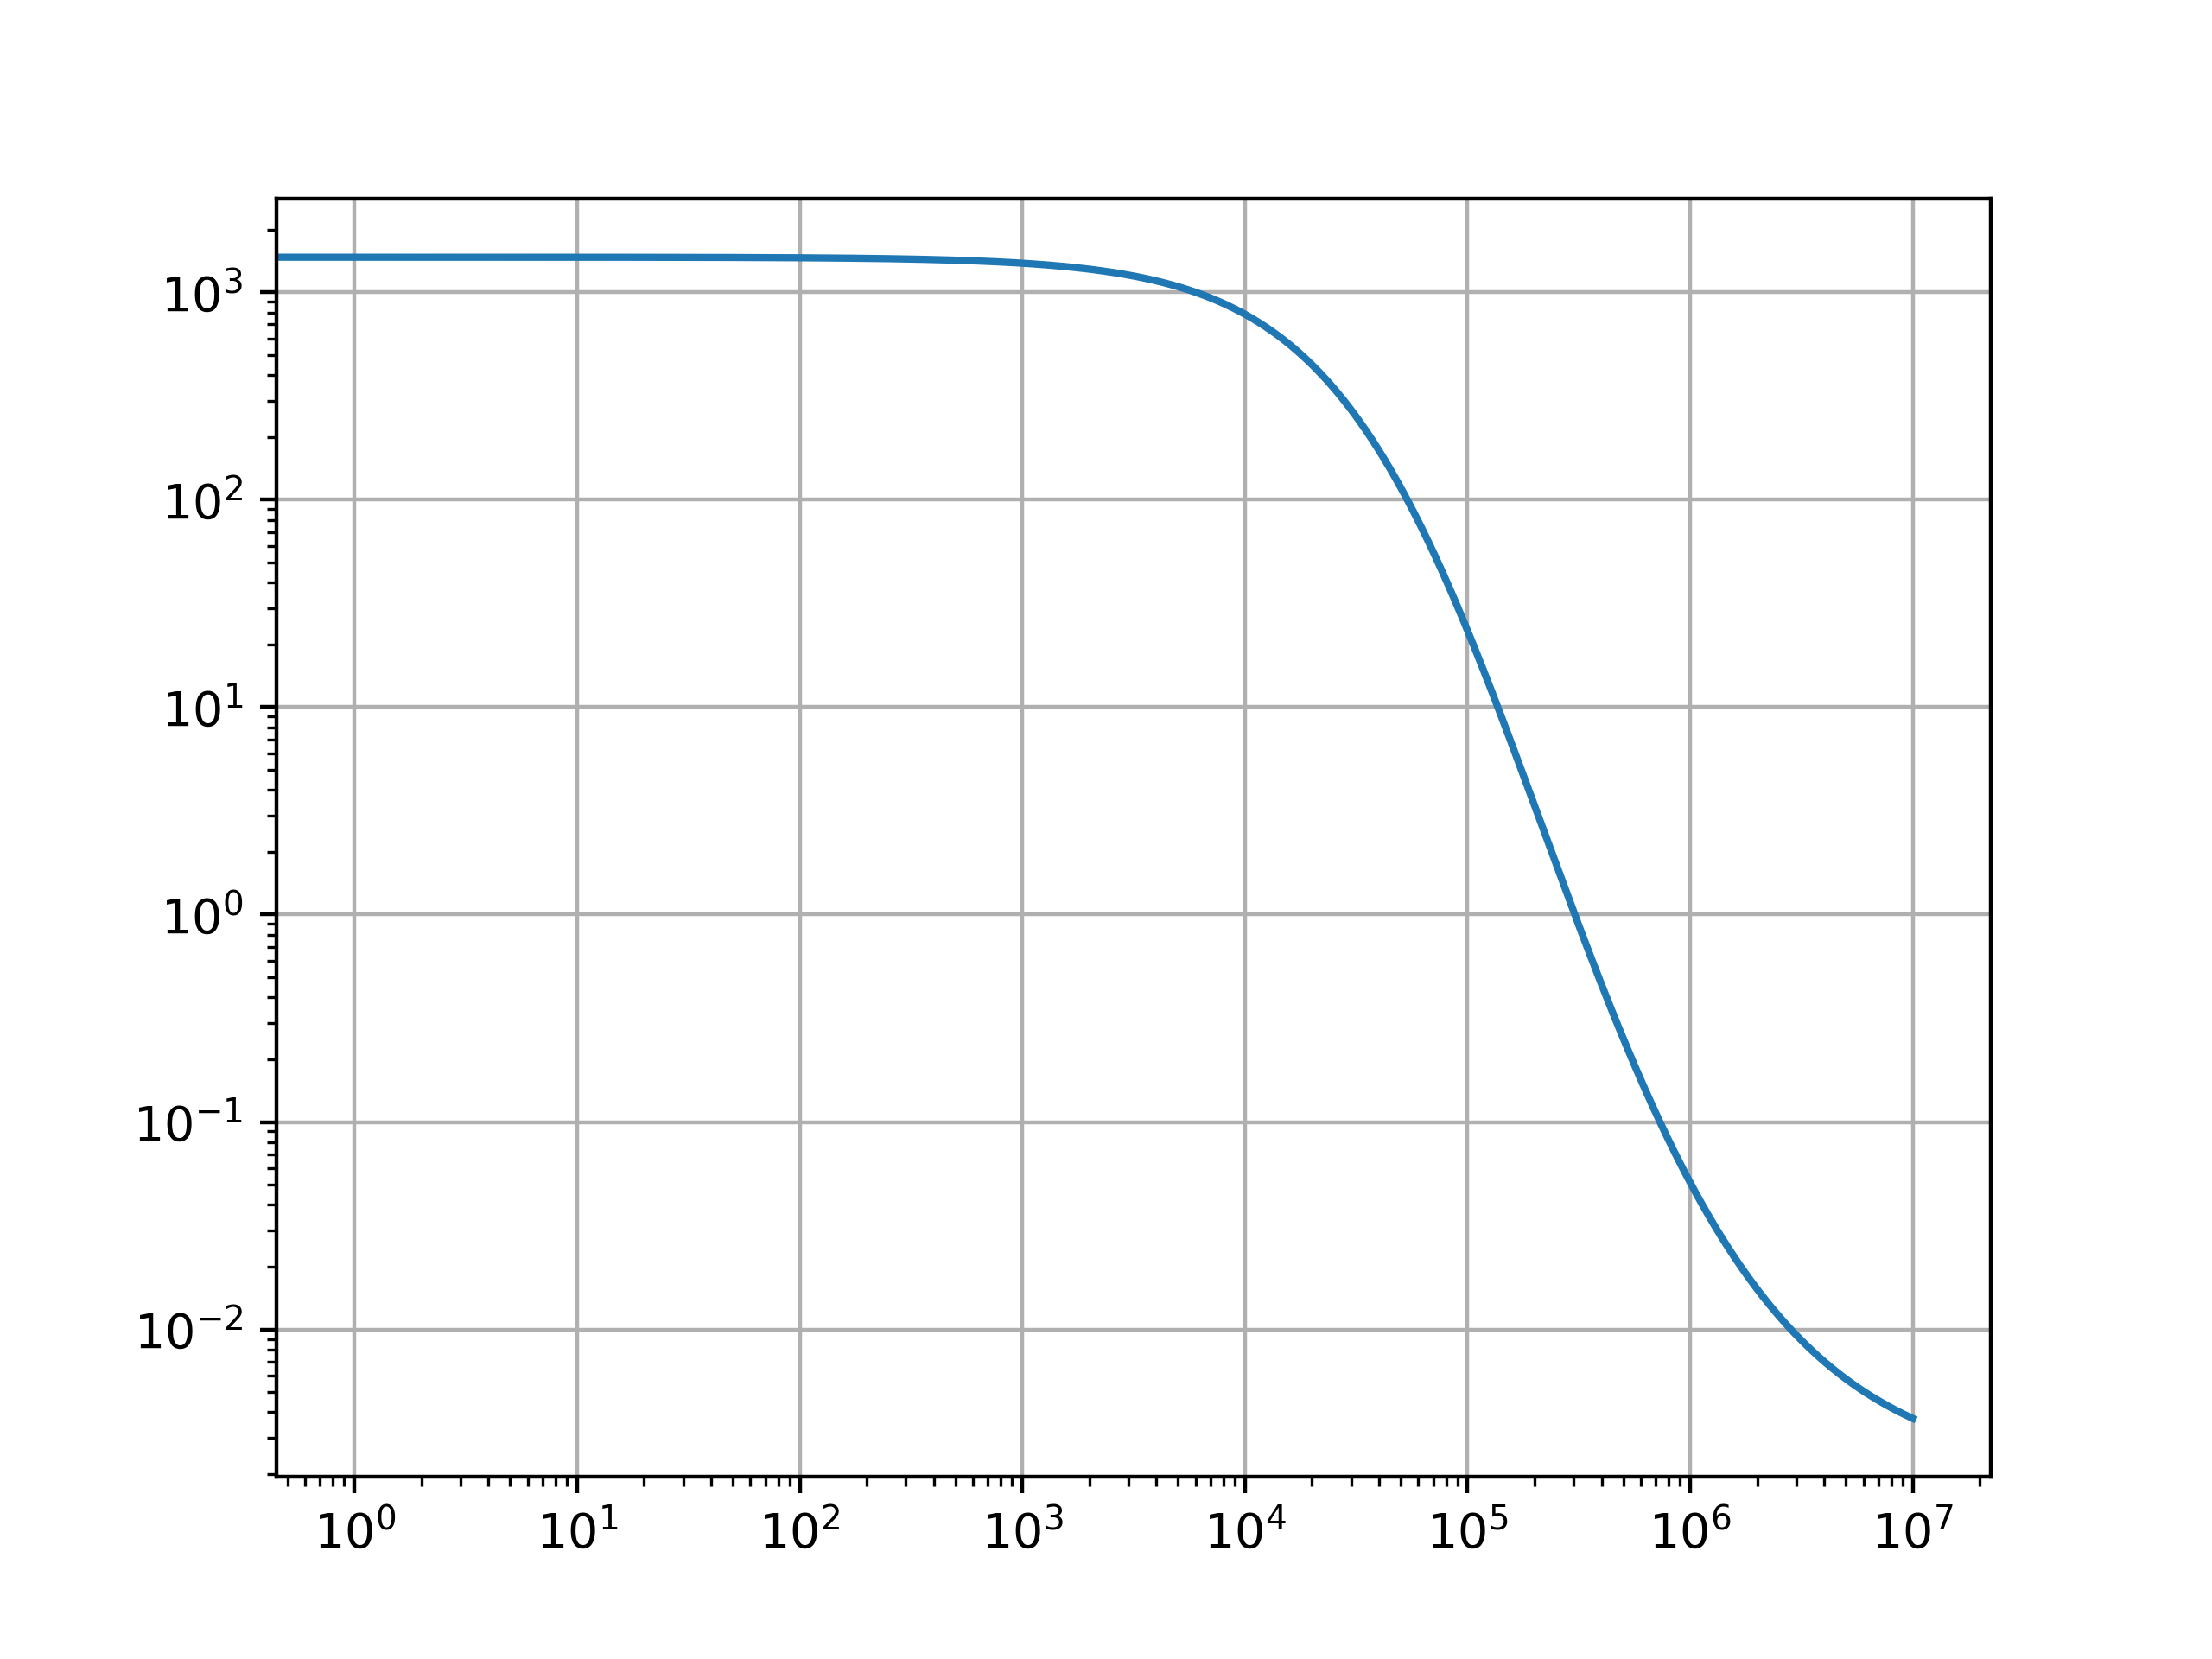
\includegraphics[width=0.8\linewidth]{1e6_6}
% \captionof{figure}{Der Entsprechende Funktionsgraph zum NFW-Profile}
% \label{fig:lookup_NFW}
% \end{center}\vspace{0.5cm}
%
% \section*{Ergebnisse}
%
% \section*{Feststellungen}
%
% \begin{itemize}
%
% \item Pellentesque\cite{stickley} eget orci eros. Fusce ultricies, tellus et pellentesque
% fringilla, ante massa luctus libero, quis tristique purus urna nec nibh.
% Phasellus fermentum rutrum elementum. Nam quis justo lectus.
%
% \item Vestibulum\cite{schwarzmeier07} sem ante, hendrerit a gravida ac, blandit quis magna.
%
% \item Donec sem metus, figureacilisis at condimentum eget, vehicula ut massa. Morbi
% consequat, diam sed convallis tincidunt, arcu nunc.
%
% \item Nunc at convallis urna. isus ante. Pellentesque condimentum dui. Etiam
% sagittis purus non tellus tempor volutpat. Donec et dui non massa tristique adipiscing.
%
% \end{itemize}
%
% \section*{Zukunft}
%
% \nocite{*} % Print all references regardless of whether they were cited in the poster or not
% \bibliographystyle{plain} % Plain referencing style
% \bibliography{poster} % Citation database is inside poster.bib
%
% \section*{Danksagungen}
%
% Hier möchte ich mich bei Tim Tugendhat und Konstantin Bosbach bedanken ohne die
% das Praktikum in Heidelberg nicht möglich gewesen wäre.
%
% \end{multicols}
% \end{document}
